\section{The \pktlanguage compiler}
\label{s:compiler}

%TODO: Do we need to mention anywhere that we do some limited dead-code removal
% and expression propagation (a generalized version of copy propagation).
% I guess these are a little pointless ...

%TODO: Help! Footnotes are inverted.
%TODO: Mention copy / expression propagation somewhere

%TODO: Mihai: Mention how the complex atoms could be used to carry out stateless
%operations as well by reducing the number of stages.
\begin{figure*}[!t]
  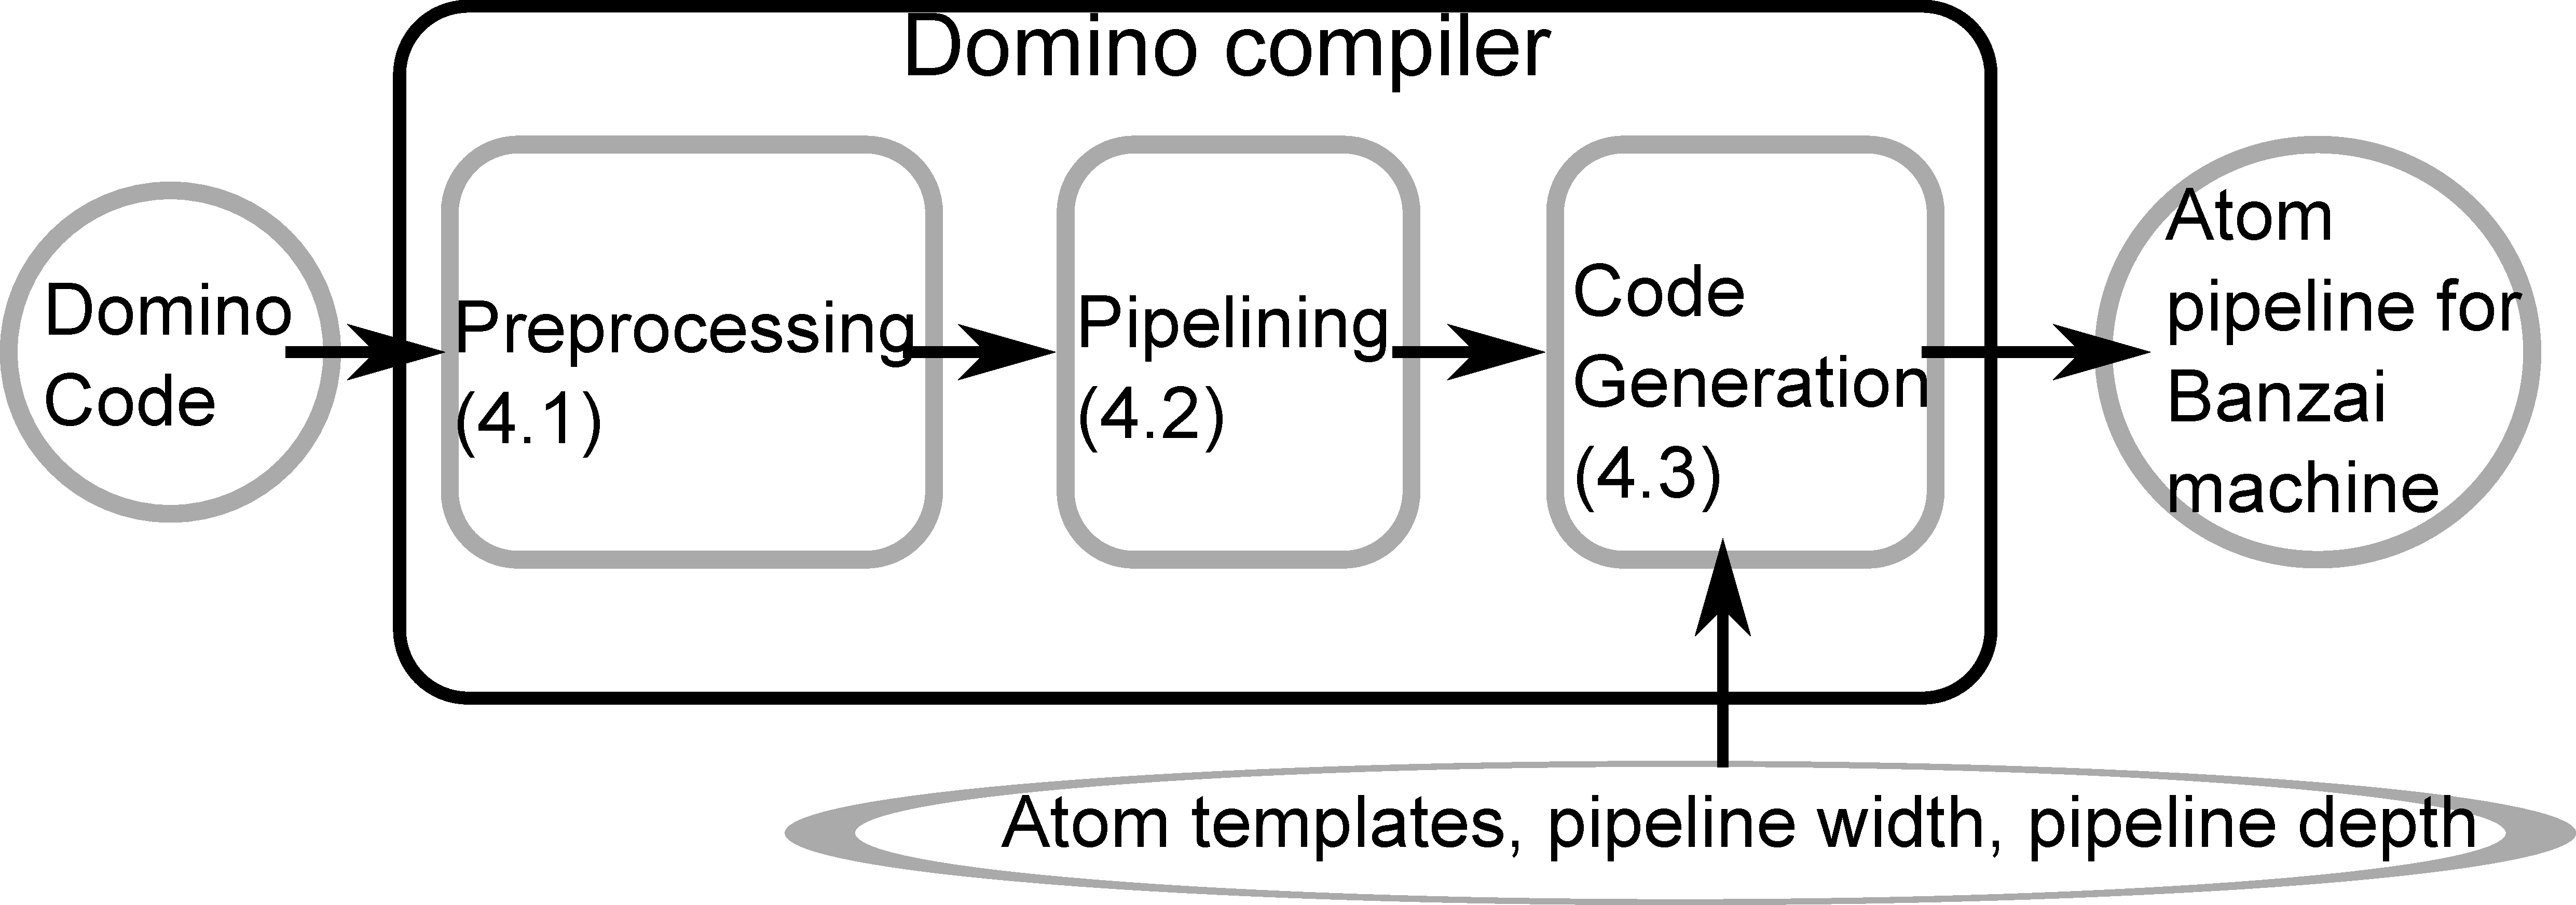
\includegraphics[width=\textwidth]{compiler.pdf}
  \caption{Passes in the \pktlanguage compiler}
\end{figure*}

\begin{figure*}[!t]
  \begin{minipage}{0.47\textwidth}
  \begin{small}
  \begin{lstlisting}[style=customc]
  if (@\textcolor{blue}{pkt.arrival - \\
      last\_time[pkt.id] \\
      > THRESHOLD}@) {
    saved_hop[pkt.id] = pkt.new_hop;
  }
  \end{lstlisting}
  \end{small}
  \end{minipage}
  \begin{minipage}{0.53\textwidth}
  \begin{small}
  \begin{lstlisting}[style=customc]
  @\textcolor{blue}{pkt.tmp = pkt.arrival - \\
            last\_time[pkt.id] \\
            > THRESHOLD}@;
  saved_hop[pkt.id] = @\textcolor{blue}{pkt.tmp}@ ? @\textcolor{blue}{// Rewritten}@
                      pkt.new_hop :
                      saved_hop[pkt.id];
  \end{lstlisting}
  \end{small}
  \end{minipage}
\caption{Conversion to straight-line code}
\label{fig:if_convert}
\end{figure*}

\begin{figure*}[!t]
  \begin{minipage}{0.43\textwidth}
  \begin{small}
  \begin{lstlisting}[style=customc]
pkt.id = hash2(pkt.sport,
               pkt.dport)
         % NUM_FLOWLETS;
...
@\textcolor{blue}{last\_time[pkt.id] = pkt.arrival;}@
...
  \end{lstlisting}
  \end{small}
  \end{minipage}
  \begin{minipage}{0.61\textwidth}
  \begin{small}
  \begin{lstlisting}[style=customc]
pkt.id = hash2(pkt.sport,         // Read flank
               pkt.dport)
         % NUM_FLOWLETS;
pkt.last_time = last_time[pkt.id];// Read flank
...
@\textcolor{blue}{pkt.last\_time = pkt.arrival; // Rewritten}@
...
last_time[pkt.id] = pkt.last_time;// Write flank
  \end{lstlisting}
  \end{small}
  \end{minipage}
  \caption{Adding read and write flanks}
\label{fig:stateful_flanks}
\end{figure*}

\begin{figure*}[!t]
  \begin{minipage}{\textwidth}
  \begin{minipage}{0.43\textwidth}
  \begin{small}
  \begin{lstlisting}[style=customc]
@\textcolor{blue}{pkt.id}@ = hash2(pkt.sport,
              pkt.dport)
              % NUM_FLOWLETS;
@\textcolor{blue}{pkt.last\_time}@ = last_time[@\textcolor{blue}{pkt.id}@];
...
@\textcolor{blue}{pkt.last\_time}@ = pkt.arrival;
last_time[@\textcolor{blue}{pkt.id}@] = @\textcolor{blue}{pkt.last\_time}@;
  \end{lstlisting}
  \end{small}
  \end{minipage}
  \begin{minipage}{0.57\textwidth}
  \begin{small}
  \begin{lstlisting}[style=customc]
  @\textcolor{blue}{pkt.id0}@ = hash2(pkt.sport, @\textcolor{blue}{// Rewritten}@ @\label{line:assign}@
               pkt.dport)
               % NUM_FLOWLETS;
@\textcolor{blue}{pkt.last\_time0}@ = last_time[@\textcolor{blue}{pkt.id0}@];  @\textcolor{blue}{// Rewritten}@
...
@\textcolor{blue}{pkt.last\_time1}@ = pkt.arrival;  @\textcolor{blue}{// Rewritten}@
last_time[@\textcolor{blue}{pkt.id0}@] = @\textcolor{blue}{pkt.last\_time1}@;  @\textcolor{blue}{// Rewritten}@
  \end{lstlisting}
  \end{small}
  \end{minipage}
  \caption[title]{SSA transformation\footnote{We rename all assignments, not just reassignments (such as line~\ref{line:assign}) because reads could precede an assignment.}}
  \label{fig:ssa}
\end{minipage}
\end{figure*}
\begin{figure*}[!t]
\begin{minipage}{\textwidth}
\begin{lstlisting}[style=customc]
pkt.id            = hash2(pkt.sport, pkt.dport) % NUM_FLOWLETS; @\label{line:id}@
pkt.saved_hop     = saved_hop[pkt.id]; @\label{line:stateRead}@
pkt.last_time     = last_time[pkt.id];
pkt.new_hop       = hash3(pkt.sport, pkt.dport, pkt.arrival) % NUM_HOPS; @\label{line:newhop}@
pkt.tmp           = pkt.arrival - pkt.last_time;
pkt.tmp2          = pkt.tmp > THRESHOLD;
pkt.next_hop      = pkt.tmp2 ? pkt.new_hop : pkt.saved_hop;
saved_hop[pkt.id] = pkt.tmp2 ? pkt.new_hop : pkt.saved_hop; @\label{line:stateWrite}@
last_time[pkt.id] = pkt.arrival;
\end{lstlisting}
\caption[title2]{Flowlet switching in three-address
code.\footnote{Lines~\ref{line:id} and ~\ref{line:newhop}) are flipped relative
to Figure~\ref{fig:flowlet}a because pkt.id is an array index expression and is
moved into the read flank.}}
\label{fig:three_address}
\end{minipage}
\vspace{-0.5cm}
\end{figure*}

The \pktlanguage compiler borrows liberally from the compiler
literature~\cite{muchnik}. However, no prior work that we know of synthesizes
compiler techniques in the same manner---prompting us to write the \pktlanguage
compiler in the first place. Further, as we illustrate throughout this section,
constraining \pktlanguage for deterministic performance has a happy side
effect: it allows us to considerably simplify the techniques in \pktlanguage's
compiler relative to their use in mainstream compilers. Because \pktlanguage's
syntax is based on C, we use clang's library interface~\cite{libclang} to
generate an Abstract Syntax Tree (AST) for packet transactions written in
\pktlanguage. The remaining compiler passes operate on this AST. Throughout
this section, we use flowlet switching from Figure~\ref{fig:flowlet}a as a
running example to demonstrate compiler passes. While we rename variables for
readability, the code output by the \pktlanguage compiler after each pass isn't
materially different from the version presented here.

\subsection{If-conversion to straight-line code}
A packet transaction's body can contain if-else statements that alter control
flow and complicate dependence analysis. As an example, we refer the reader to
the pseudocode of the CoDel algorithm available at~\cite{codel_code}. We
eliminate if-else statements by transforming them into the C conditional
operator, starting from the innermost if statements and recursing outwards
(Figure~\ref{fig:if_convert}). This procedure is called
if-conversion~\cite{if_conversion}. It is much simpler in \pktlanguage because
only if-else statements alter control flow in \pktlanguage and all other control
transfer is forbidden.  This transformation creates
straight-line code, where control passes sequentially without branching.
Straight-line code simplifies the rest of the compiler, like computing the
static single-assignment form(\S\ref{ss:ssa}).

%TODO: Ask Alvin how this can be fixed.
\subsection{Converting to load/store form}

We next identify both array and scalar state variables used in a packet
transaction, such as \texttt{last\_time} and \texttt{saved\_hop} in
Figure~\ref{fig:flowlet}. For each state variable, we create a \textit{read
flank} to read the state variable into a temporary packet field. For an array,
we also move the index expression into the read flank, exploiting the fact that
only one array index is accessed by each packet in valid \pktlanguage programs.
Then, throughout the packet transaction, we the state variable with the packet
temporary, and create a \textit{write flank} to write the packet temporary back
into the state variable.  Figure ~\ref{fig:stateful_flanks} illustrates this
transformation on a fragment.  After this pass, the code resembles code for a
load-store architecture~\cite{load_store}: state variables only support reads
and writes; arithmetic happens on packet variables.  Restricting operations on
state variables simplifies their treatment during code partitioning
(\S\ref{ss:partitioning}).

\subsection{Renaming variables to SSA}
\label{ss:ssa}

We next convert to static single-assignment form (SSA)~\cite{ssa}, an
intermediate form used by many compilers~\cite{tree_ssa, llvm}, where every
variable is assigned exactly once. To compute the SSA, we replace every
definition of a packet variable with a new packet variable and propagate this
new packet variable until the next definition of the same packet variable.
State variables are already in SSA form: after their flanks have been added,
every state variable is written exactly once in the write flank.  While general
algorithms for computing the SSA are fairly involved~\cite{ssa}, \pktlanguage's
SSA computation is simpler because it operates on straight-line code.  SSA
simplifies further analysis because every variable is assigned exactly once.
This implies that there are no Write-After-Read or Write-After-Write
dependencies. Only Read-After-Write dependencies remain, simplifying dependency
analysis during code partitioning (\S\ref{ss:partitioning}).

\subsection{Flattening to three-address code}
We next transform into three-address code~\cite{tac}, where all instructions
are either reads / writes into stateful variables or carry out packet
manipulations of the form: \texttt{pkt.f1 = pkt.f2 op pkt.f3;} where
\texttt{op} includes all arithmetic, logical, and relational operators. We also
allow either pkt.f2 or pkt.f3 to be function call to an intrinsic, because we
assume these are supported in hardware. To generate three-address code, we
flatten expressions that are not already legal in three-address code, by
introducing enough temporaries (Figure~\ref{fig:three_address}).

Flattening expressions may result in temporaries that compute the same
subexpression. For instance, if the two statements \texttt{x = a * 5 + b;} and
\texttt{x = a * 5 + c;} were flattened, the subexpression \texttt{a * 5} would
be computed by two temporaries. We eliminate such temporaries using
common subexpression elimination~\cite{cse}.

\subsection{Code partitioning to codelets}
\label{ss:partitioning}
At this point, the code is still sequential. Code partitioning turns sequential
code into a pipeline of \textit{codelets}, where each codelet is a small
sequential block of three-address code statements. We do so by exploiting
parallelism within and across pipeline stages.  Subsequently, we map each
codelets one-to-one to atoms provided by a particular \absmachine
machine~(\S\ref{ss:code_gen}), returning a compiler error if any codelet
doesn't map to an atom provided by the hardware.

To partition code into codelets, we carry out the following steps:
\begin{CompactEnumerate}
  \item Create a node for each statement (Figure~\ref{fig:three_address}) in
    the packet transaction after expression flattening.
  \item Create a bidirectional edge between nodes N1 and N2 where N1 is a read from a
    state scalar / state array and N2 is a write into the same state scalar /
    state array. This step captures the constraint that state is internal to an
    atom in \absmachine. Because state variables don't occur in any
    instructions besides reads and writes, this is all we need to do to handle
    state variables.
  \item Create an edge (N1, N2) for every pair of nodes N1, N2 where N2 reads
    a variable written by N1. We only check read-after-write dependencies because
    control dependencies turn into data dependencies when generating straight-line
    code. Further, the use of SSA removes all write-after-read and write-after-write
    dependencies.
  \item Generate strongly connected components (SCCs) of the resulting graph
    (Figure~\ref{fig:partitioning}a) and condense the SCCs to to create a directed
    acyclic graph (DAG) (Figure~\ref{fig:partitioning}b). This step captures the
    constraint that all operations on state variables (read, write, and modify)
    must reside within the same atom because state is local to an atom.
  \item Schedule the resulting DAG using critical path
    scheduling~\cite{crit_path_sched}, creating a new pipeline stage every time
    one operation needs to follow another (Figure~\ref{fig:flowlet}b).
\end{CompactEnumerate}
At this point, the resulting codelet pipeline (Figure~\ref{fig:flowlet}b)
implements the packet transaction.  Further, the codelets themselves have a
stylized form.  Codelets that don't manipulate state contain exactly one
three-address code instruction. Codelets that manipulate state contain at least
two statements: a read from a state variable and a write to a state variable.
They optionally consist of one or more updates to the state variable through
packet temporaries.

\begin{figure*}[!t]
\begin{minipage}{0.5\textwidth}
  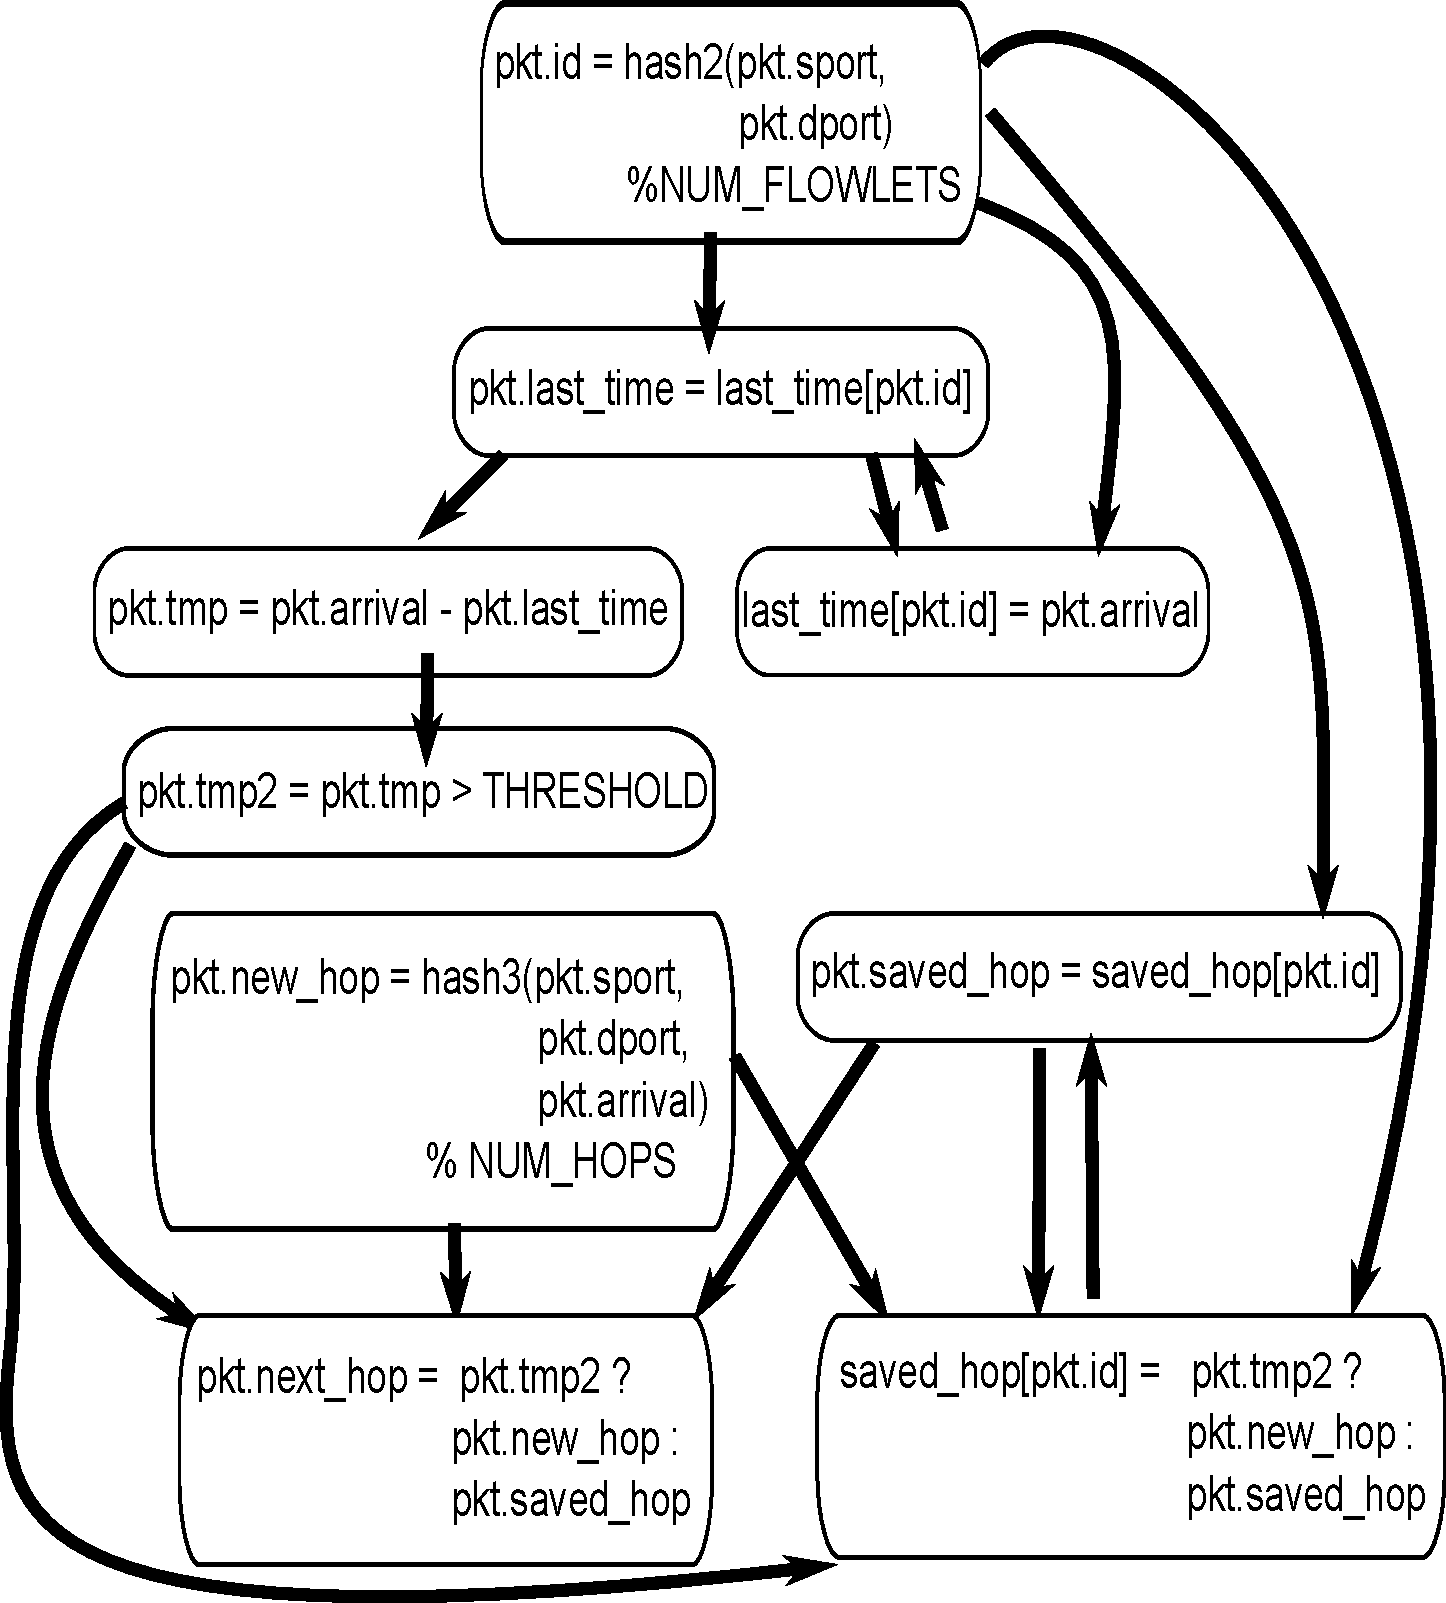
\includegraphics[width=\columnwidth]{deps.pdf}
\end{minipage}
%
\vrule\quad
%
\begin{minipage}{0.5\textwidth}
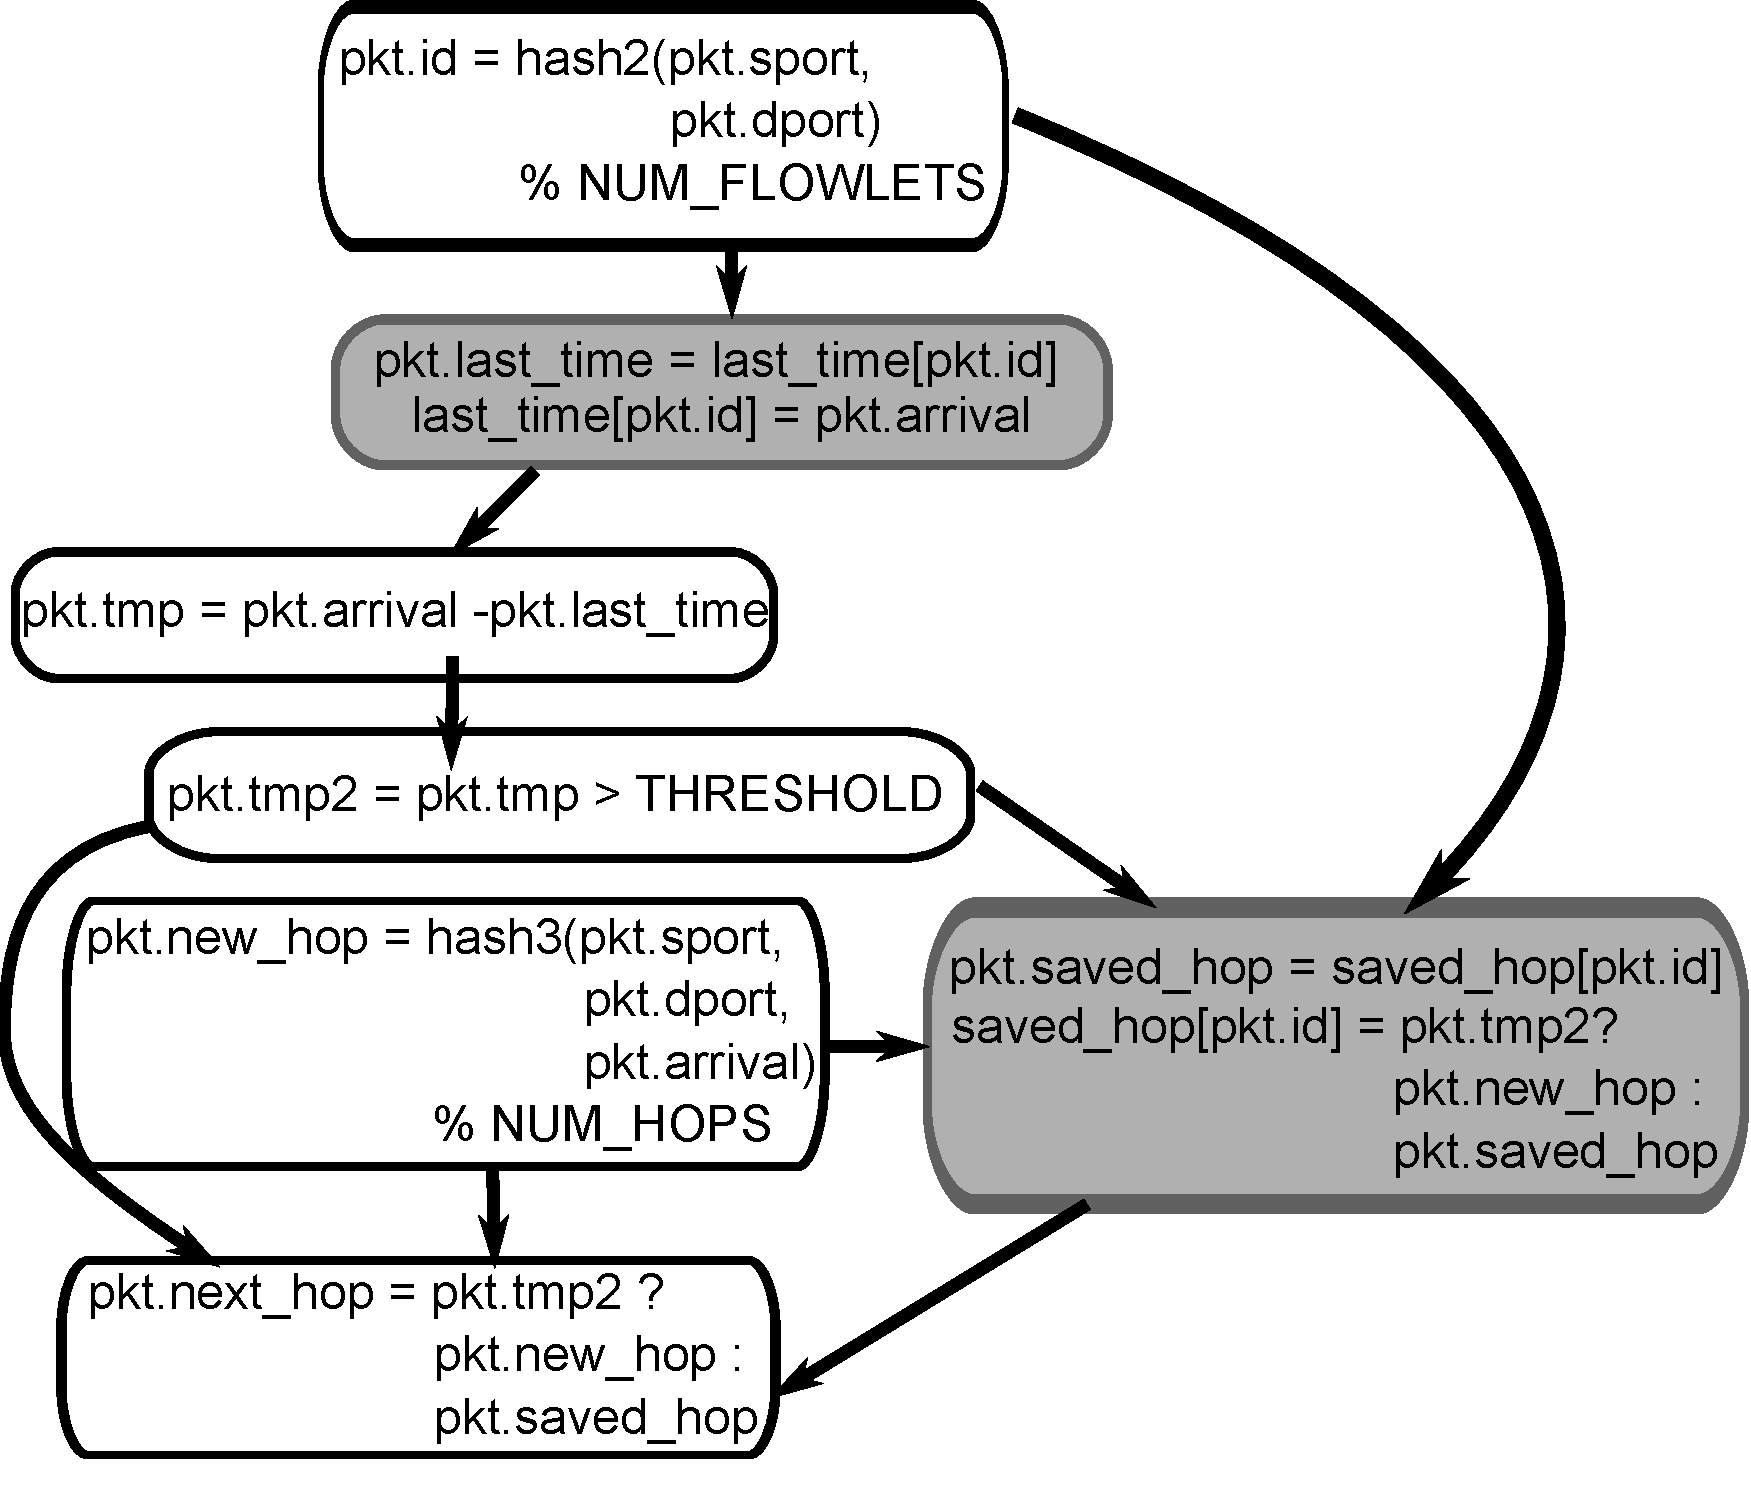
\includegraphics[width=\columnwidth]{scc.pdf}
\end{minipage}
\caption{Dependency graph (a) before and (b) after condensing strongly connected components}
\label{fig:partitioning}
\end{figure*}

\subsection{Mapping a codelet to an atom}
\label{ss:code_gen}
Next, we determine how the codelets created by code partitioning in the
previous step map one-to-one to atoms provided by the \absmachine machine. We
consider codelets that do and don't manipulate state separately because we
handle each differently.

\textbf{Stateless codelets}
Expression flattening generates stateless codelets that each have only one
statement in three-address code form (e.g. any of the unshaded boxes in
Figure~\ref{fig:flowlet}b). For this paper, we assume that all \absmachine
machines support stateless atoms that correspond to a single statement in
three-address code form. P4's primitives~\cite{p4spec} and RMT's VLIW action
set~\cite{rmt} both resemble this form. Under this assumption, mapping a
stateless codelet is simple: each stateless codelet has exactly one
three-address code statement, which is equivalent to an atom provided by the
\absmachine machine. If the \absmachine machine supports stateless atoms beyond
a single three-address code instruction, our approach is still correct,
although suboptimal. For instance, if the \absmachine machine supports a
multiply-and-accumulate atom~\cite{mac}, expression flattening would generate
two atoms (one each for the multiply and accumulate), where one suffices.

\textbf{Stateful codelets}
Stateful codelets have multi-line bodies that need to execute atomically. For
instance, updating the state variable \texttt{saved\_hop} in
Figure~\ref{fig:flowlet}b requires a read, followed by a conditional write.  It
is not apparent whether these codelets can be mapped to an available atom. We
develop a general technique to determine the implementability of such stateful
codelets, given as input the stateful atom template provided by the \absmachine
machine.

An atom template defines a space of possible computations such as different
permissable ALU operations.  The exact computation is selected by
\textit{configuring} the atom. The codelet is a specification that is to be
checked for functional equivalence against one of the atom configurations
supported by the atom template. We need to \textit{synthesize} the atom's
\textit{configuration}, given an \textit{atom template} describing the atom's
functionality.

This is the realm of syntax-guided program synthesis~\cite{sgsyn}, where the
programmer supplies a partial program or template (hence the term
syntax-guided) with missing details, and a specification. A \textit{program
synthesis tool} then synthesizes these details in the partial program so that
it matches up with the specification. One such program synthesis tool is
SKETCH~\cite{bitstreaming, sketch_asplos, sketch_manual}, which allows the
programmer to specify a partial program with \textit{holes} that are then
``filled in'' by SKETCH to match the specification (Figure~\ref{fig:sketch}).

\begin{figure}[!b]
  \begin{center}
  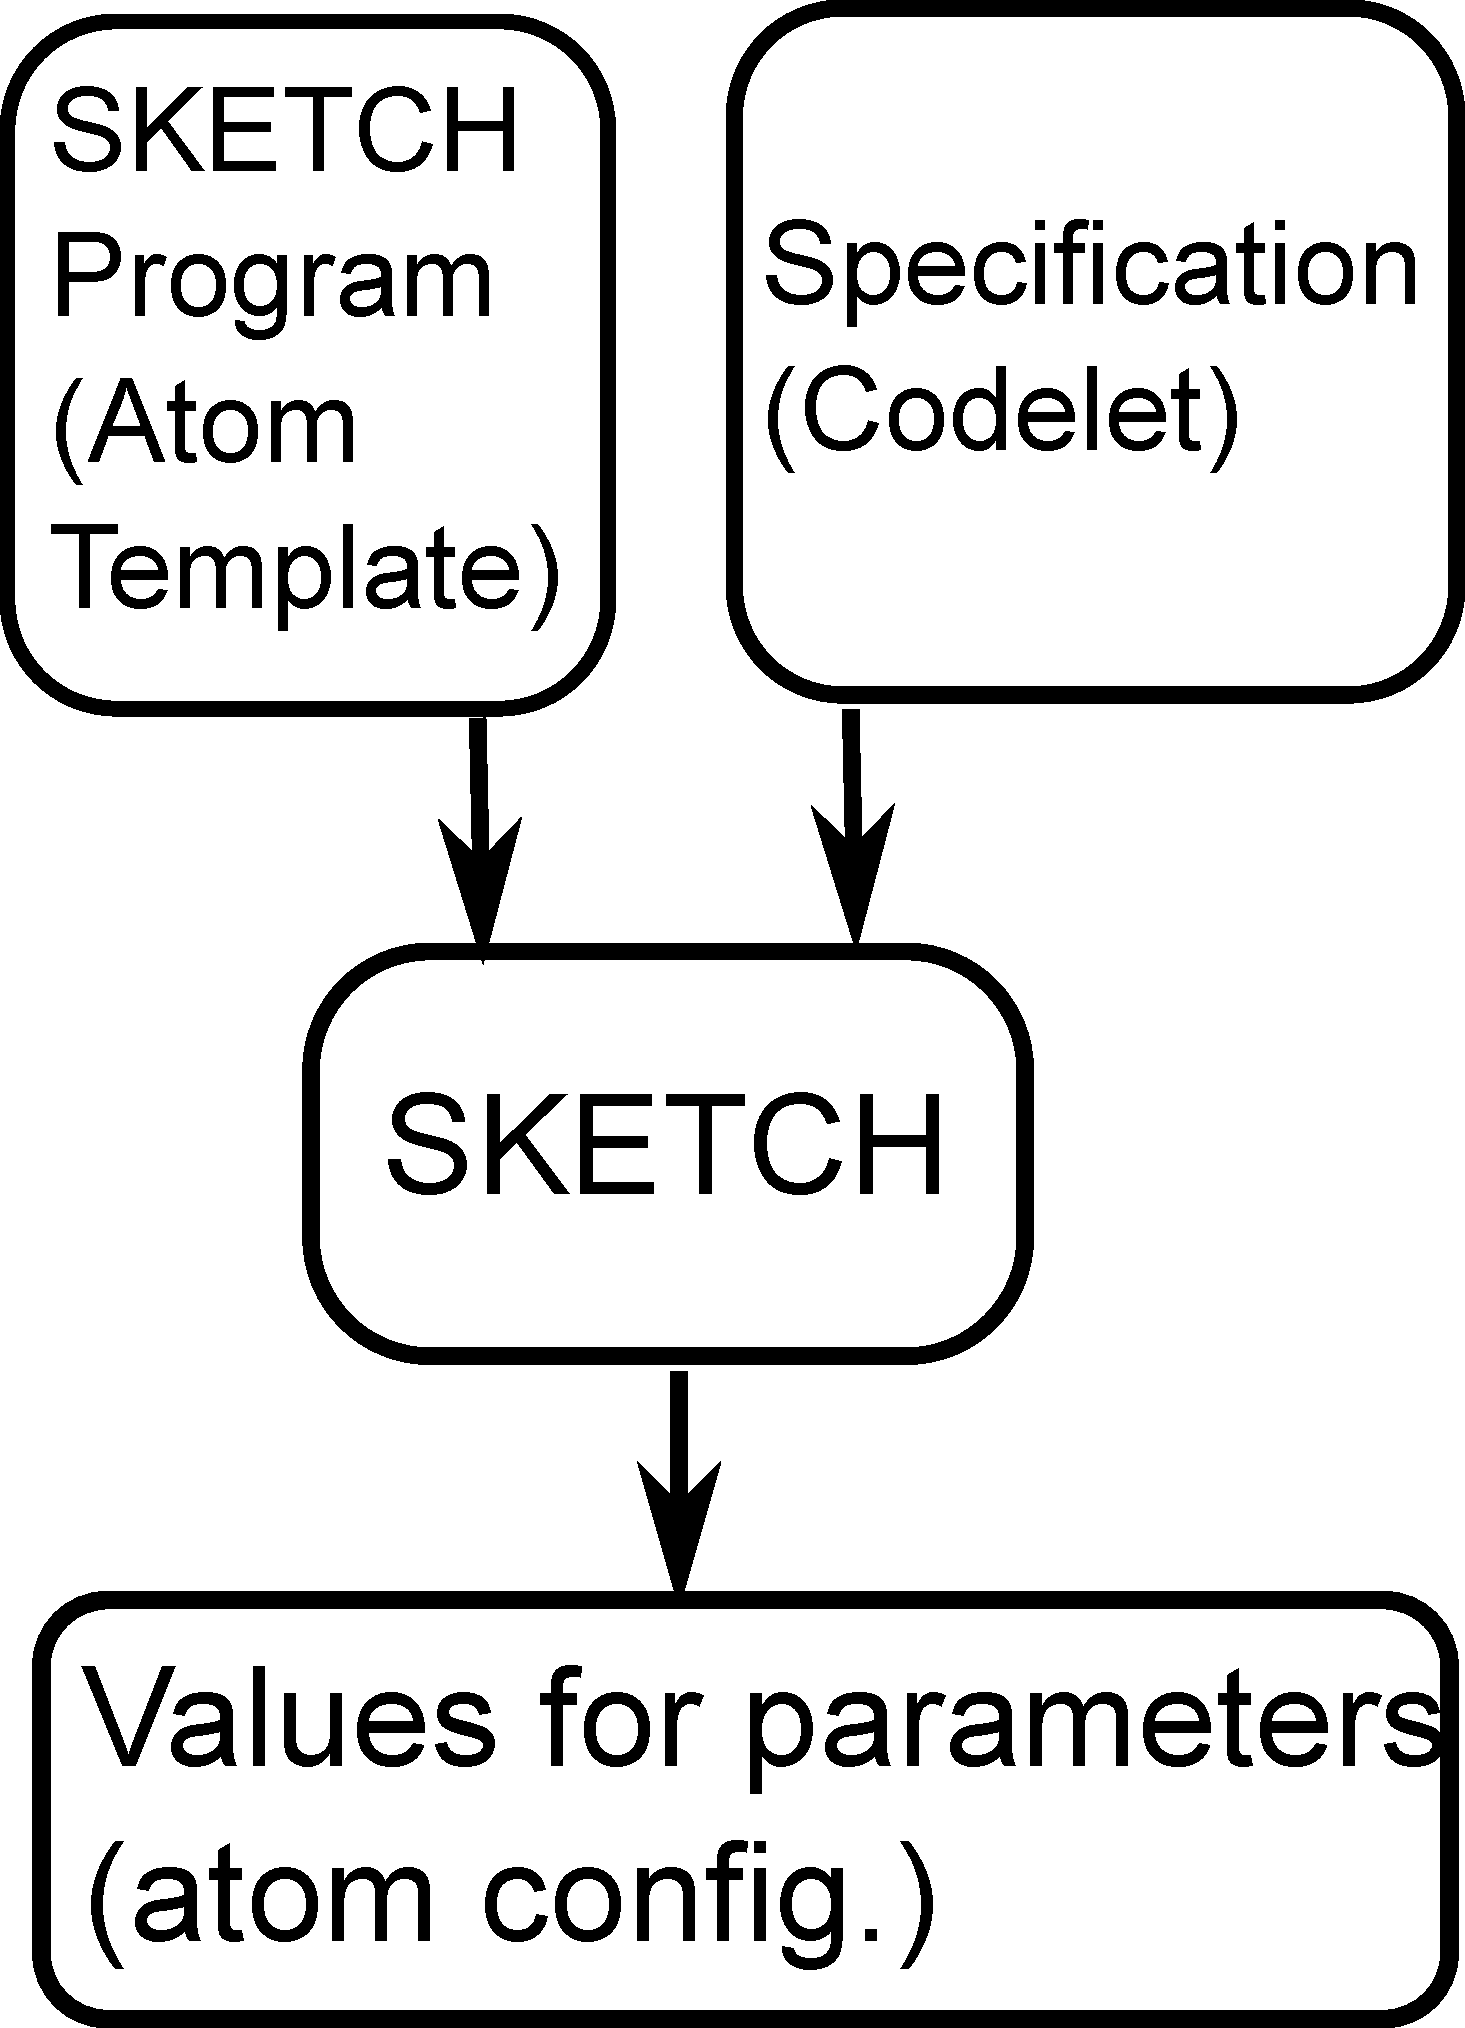
\includegraphics[width=0.4\columnwidth]{sketch.pdf}
  \caption{Overview of SKETCH and its application to atom configuration}
  \label{fig:sketch}
  \end{center}
\end{figure}

\begin{figure}[h]
  \begin{minipage}{0.4\columnwidth}
  \begin{center}
  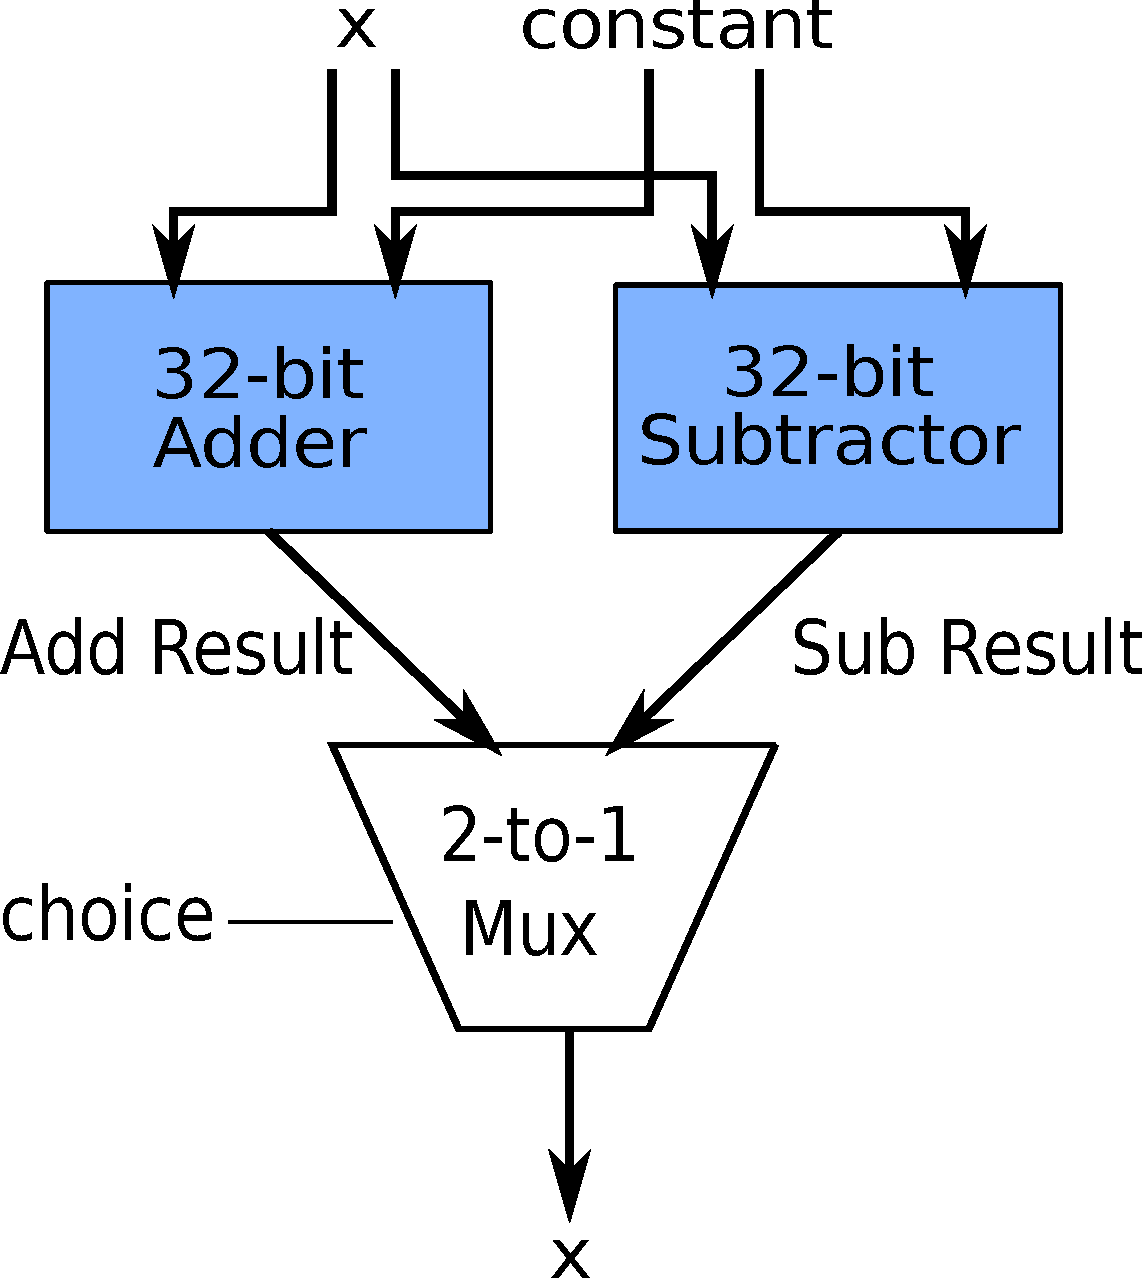
\includegraphics[width=\columnwidth]{circuit.pdf}
  \end{center}
  \end{minipage}
  \begin{minipage}{0.55\columnwidth}
  \begin{center}
  \begin{lstlisting}
  bit choice = ??(1);
  int constant = ??(5);
  if (bit) {
    x = x + constant;
  } else {
    x = x - constant;
  }
  \end{lstlisting}
  \end{center}
  \end{minipage}
\caption{\small (a) Circuit for an atom that can either add or subtract a
constant from a state variable.  (b) Circuit's representation in SKETCH.
Each ``??(n)'' represents a hole that can be filled in with values in
  $[0, 2^n -1]$.}
\label{fig:alu_in_sketch}
\end{figure}

We use SKETCH to solve the atom configuration problem.  Consider an atom
template that models an ALU (Figure~\ref{fig:alu_in_sketch}a) taking two
configuration parameters: an opcode, \texttt{choice}, specifying an addition or
subtraction operation, and a 5-bit positive constant, \texttt{constant}.  The ALU's
functionality is to add or subtract this constant from one state variable. This
ALU can be represented by the SKETCH partial program given in
Figure~\ref{fig:alu_in_sketch}b.

Assume we want to map the codelet x=x+1 to this atom. The codelet is then fed
into SKETCH as the desired specification and the atom template is fed into
SKETCH as the partial program (Figure~\ref{fig:sketch}). SKETCH will configure
the atom template by setting \texttt{choice} to 0 and \texttt{constant} to 1.
In contrast, if the codelet x = x * x was supplied as the specification, SKETCH
will return an error because the specification cannot be mapped to any of the
atom's computations. We don't describe the algorithms underlying SKETCH because
we treat SKETCH as a blackbox in the \pktlanguage compiler. The interested
reader is referred to~\cite{bitstreaming, sketch_asplos} for a more detailed
treatment of these topics.

Using SKETCH to represent atom templates allows us to express the behavior of
diverse atoms (Table~\ref{tab:templates}) using a natural imperative syntax.
Because different \absmachine machines only differ in the atoms they provide,
employing SKETCH for atom configuration lets us build a retargetable
compiler~\cite{lcc} with little target-dependent work beyond specifying each
target's atoms as partial programs in SKETCH.

\subsection{Verifying compilations}
\label{ss:verification}

We next describe our testing infrastructure to verify that the
compilation is correct i.e. the externally visible behavior of the packet
transaction (Figure~\ref{fig:flowlet}a) is indistinguishable from its pipelined
implementation (Figure~\ref{fig:flowlet}b). We verify correctness by feeding in
the same set of test packets to both the packet transaction and its
implementation and comparing the outputs from both programs on the set of
externally visible fields.

To create test packets, we scan the packet transaction and generate the set of
all fields read from or written to by the transaction. We initialize each field
by sampling independently and uniformly from the space of all 32-bit signed
integers.  To compare outputs from the packet transaction and its
implementation, we track renames that occur because of SSA and compare each
output field in the transactional form with its last rename in the
implementation. We then feed the same test packets to both the specification
and implementation and compare outputs at the end of the pipeline. This lets us
quickly ``spot check'' our compilations and helped discover a few compiler bugs
during development.

\subsection{Targeting real switches}
\label{ss:real}
\pktlanguage doesn't yet generate code for actual hardware. We initially
considered compiling \pktlanguage to P4. However, P4 currently doesn't support
sequential execution within a pipeline stage---required to correctly execute
the codelets/atoms produced by \pktlanguage. Based on this work, we have
submitted a proposal for sequential execution~\cite{p4-semantics} to the P4
language consortium. In the future, if P4 supports sequential execution,
\pktlanguage could target P4 as a backend, which would then allow \pktlanguage
to target programmable switches by leveraging ongoing work~\cite{netronome,
xilinx,lavanya_compiler} in P4 compilation.
